\textbf{See the instruction for questions \inteval{\value{question}+1} to \inteval{\value{question}+2}.}

\begin{center}
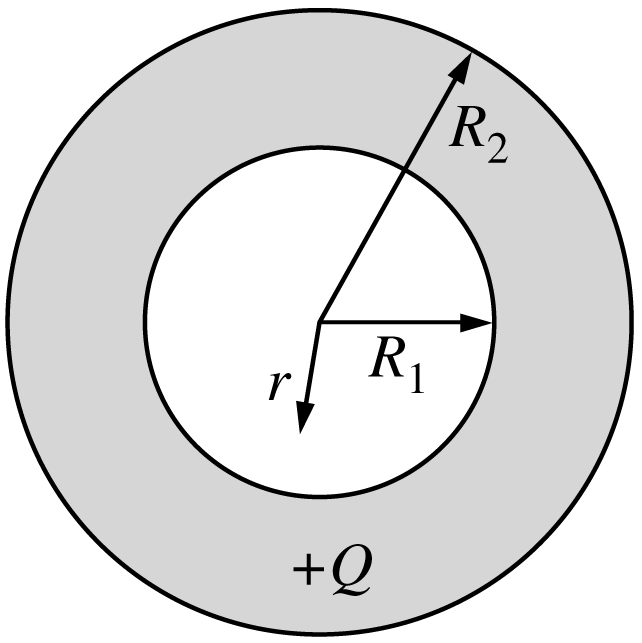
\includegraphics[scale=0.2]{images/img-007-008.png}
\end{center}

A charge $+Q$ is uniformly distributed throughout a nonconducting spherical shell of inner radius $R_{1}$ and outer radius $R_{2}$, as shown above. The electric field is determined at a distance $r$ from the center of the spherical shell.

% Multiple Choice Question 12
\begin{questions}\setcounter{question}{11}\question
The electric field for $r<R_{1}$ is

\begin{oneparchoices}
\choice zero
\choice $\dfrac{1}{4 \pi \epsilon_{0}} \dfrac{Q}{R_{1}^{2}}$
\choice $\dfrac{1}{4 \pi \epsilon_{0}} \dfrac{Q}{R_{2}^{2}}$
\choice $\dfrac{1}{4 \pi \epsilon_{0}} \dfrac{Q}{\left(R_{2}-R_{1}\right)^{2}}$
\choice $\dfrac{1}{4 \pi \epsilon_{0}} \dfrac{Q}{R_{2}^{2}-R_{1}^{2}}$
\end{oneparchoices}\end{questions}

% Multiple Choice Question 13
\begin{questions}\setcounter{question}{12}\question
The electric field for $r>R_{2}$ is

\begin{oneparchoices}
\choice $\dfrac{1}{4 \pi \epsilon_{0}} \dfrac{Q}{R_{1}^{2}}$
\choice $\dfrac{1}{4 \pi \epsilon_{0}} \dfrac{Q}{R_{2}^{2}}$
\choice $\dfrac{1}{4 \pi \epsilon_{0}} \dfrac{Q}{r^{2}}$
\choice $\dfrac{1}{4 \pi \epsilon_{0}} \dfrac{Q}{r^{2}-R_{2}^{2}}$
\choice $\dfrac{1}{4 \pi \epsilon_{0}} \dfrac{Q}{R_{2}^{2}-R_{1}^{2}}$
\end{oneparchoices}\end{questions}

